\scanpage{56}
\mspage{2}

en série qui commence par
\[
a_n z^n\text{ ---}\qquad n>0,\ a_n\ne0\qquad(\mathrm{OPS}\ x=0)
\]
on voit tout de suite que l'on doit avoir $n=1$ ---

% slanted
\margin{Noter : \uline{indétermination} d'une carte loc. au bord : modulo chgt. de coordonnées par un germe de fonction analytique \uuline{réelle}.}

[\uline{Thm 2} Équiv. de la cat. des surfaces conformes à bord \inserted{compactes,} avec celle des courbes alg. propres lisses sur $\mathbb R$.]

% slanted
\margin{\uline{NB} À partir d'ici $H$ désigne le demi-plan \uline{fermé} $\{z\in\mathbb C\mid\Im z\geq 0\}$}

\textcircled{\unsure{2|b}} \unsure{Découpe|Découpage} d'une surface conforme à bord, suivant un 1-complexe top. $K\subset X$, satisfaisant des hypothèses de régularité convenables (rectifiabilité suffit ?).

\uline{Théorème 3} La découpe $\widetilde X$, munie du \deleted{la} \deleted{structure} \inserted{faisceau} ``des fonctions \inserted{complexes} continues conformes dans $\operatorname{Int}(\tilde{\unsure{x|X}})$ ($\simeq X\smallsetminus K$), ``est'' une surface conforme à bord.

% slanted
\margin{C'est un th. du type ``uniformisation \deleted{\unsure{généralisée}} \inserted{à bord}''}

Cela revient à vérifier \deleted{deux} que \inserted{pour} tout point $\tilde x$ de $\partial\widetilde X$, il existe un voisinage \inserted{ouvert} $U$ de $x$, et un \deleted{\unsure{isom}} \inserted{homéo} de $U$ avec $H\cap\mathring{\mathbb D}$ (où $\mathbb D=\{z\in\mathbb C\mid |z|\leq 1\}$ est le disque unité de $\mathbb C$).

% slanted
\margin{\unsure{purement|revient} dans a) Cor. au thm.}

\figure{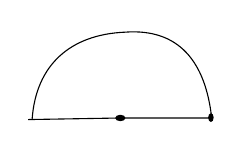
\begin{tikzpicture}[x=1cm,y=1cm]
\draw (0,0) .. controls (0.05,0.68) and (0.48,1.07) .. (1.18,1.10) .. controls (1.86,1.15) and (2.20,0.73) .. (2.28,0.01);
\draw (-0.05,-0.01) -- (1.12,0.01) -- (2.29,0.01);
\fill (1.12,0.01) ellipse (0.065 and 0.041);
\fill (2.27,0.015) ellipse (0.035 and 0.056);
\end{tikzpicture}}

Cela revient à deux choses, suivant que $x$ correspond :
% archive sheet number: 58
